% Settings for the default beamer theme
\documentclass[english, aspectratio=169]{beamer}
\usepackage[T1]{fontenc}
\usepackage[utf8]{inputenc}
\usepackage{tabularx}
\usepackage{babel}
\usepackage[ruled,vlined]{algorithm2e}
\SetAlgorithmName{Algoritmus}{algoritmus}{List of Algorithms}
\setcounter{secnumdepth}{3}
\setcounter{tocdepth}{3}

\makeatletter

\newcommand\makebeamertitle{\frame{\maketitle}}

% (ERT) argument for the TOC
\AtBeginDocument{%
  \let\origtableofcontents=\tableofcontents
  \def\tableofcontents{\@ifnextchar[{\origtableofcontents}{\gobbletableofcontents}}
  \def\gobbletableofcontents#1{\origtableofcontents}
}

% Theme settings
\usetheme{Frankfurt}
\usecolortheme{default}
\usefonttheme[onlymath]{serif}

% Template settings
\setbeamertemplate{navigation symbols}{}
\setbeamertemplate{blocks}[rounded][shadow=false]
\setbeamertemplate{title page}[default][colsep=-4bp, rounded=true, shadow=false]
\makeatother

% Define a custom darker red color
\definecolor{DarkerRed}{RGB}{139,0,0} % Adjust the RGB values as needed

% Use the newly defined color in Beamer theme elements
\setbeamercolor{structure}{fg=DarkerRed} % Changes basic structural elements to Darker Red
\setbeamercolor{title in head/foot}{bg=DarkerRed} % Changes the title in header/footer to Darker Red


\begin{document}

% Title page
\section{SVM modellek}
\title[]{Üzleti Elemzések Módszertana}
\subtitle{6. Előadás: Tartó vektor gépek}
\author[Kuknyó Dániel]{Kuknyó Dániel\\Budapesti Gazdasági Egyetem}
\date{2023/24\\2.félév}
\makebeamertitle

% Table of contents slide
\begin{frame}
\tableofcontents{}
\end{frame}

% Table of contents of the current section
\begin{frame}
\tableofcontents[currentsection]
\end{frame}

\begin{frame}{A vektorgépek mögötti intuíció}
\begin{columns}
\begin{column}{.5\textwidth}
Az SVM modellek minden esetben a \textbf{legszélesebb utat} keresik egy adathalmaz két osztálya között. Az út közepén húzódik a \textbf{döntési határ} és \textbf{az út két oldalán fekszenek a margók}.\par\medskip
Az úton kívül hozzáadott mintaegyedek nem befolyásolják a döntési határt, tehát az utat a csoportok szélén lévő mintaegyedek tartják.\par\medskip
A margó egyik oldalán $A$, a másikon pedig $B$ osztály lesz a predikció.
\end{column}
\begin{column}{.5\textwidth}
\begin{center}
\includegraphics<1>[width=7cm, height=7cm, keepaspectratio]{images/svm_1.png}
\includegraphics<2>[width=7cm, height=7cm, keepaspectratio]{images/svm_2.png}
\end{center}
\end{column}
\end{columns}
\end{frame}

\begin{frame}{Adat előkészítés}
\begin{columns}
\begin{column}{.5\textwidth}
A tartó vektor gépek nagyon szenzitívek az adatok méretezésére.
\begin{block}{Normalizálás}
A normalizálás (vagy méretezés) célja, hogy az adatkészlet különböző változóit egységes mértékrendszerbe hozza.\par\smallskip
Ennek következménye, hogy a predikcióhoz minden változó egyenlő súllyal hozzájáruljon.
\end{block}
Érdemes megfigyelni az út változását méretezés előtt és után.
\end{column}
\begin{column}{.5\textwidth}
\begin{center}
\includegraphics<1>[width=7cm, keepaspectratio]{images/svm_3.png}
\includegraphics<2>[width=7cm, keepaspectratio]{images/svm_4.png}
\end{center}
\end{column}
\end{columns}
\end{frame}

\begin{frame}{Keménymargós osztályozás}
\begin{columns}
\begin{column}{.5\textwidth}
\begin{block}{Keménymargós osztályozás}
Amennyiben áll az a feltétel, hogy minden mintaegyednek az úton kívül kell esnie, az osztályozás \textbf{keménymargós}.
\end{block}
Ez csak akkor lehetséges, amikor az adatok lineárisan szeparálhatóak. Ezenkívül a kiugró adatpontok képesek irracionálisan torzítani a modell határait.\par\smallskip 
Ennek kiküszöbölésére olyan modellre van szükség, amelyik engedélyezi a \textbf{margósértéseket}. 
\end{column}
\begin{column}{.5\textwidth}
\begin{center}
\includegraphics<1>[width=7cm, keepaspectratio]{images/svm_5.png}
\includegraphics<2>[width=7cm, keepaspectratio]{images/svm_6.png}
\end{center}
\end{column}
\end{columns}
\end{frame}

\begin{frame}{Lágymargós osztályozás}
\begin{columns}
\begin{column}{.5\textwidth}
A margósértések és a rosszul generalizáló modellek közötti optimum keresésére hivatottak a lágymargós SVM modellek. 
\begin{block}{Lágymargós osztályozás}
Olyan SVM modell, amely \textbf{engedélyezi a margósértéseket}. \textbf{A margó keménységét a $C$ hiperparaméter szabályozza.}\par\smallskip
A kisebb $C$ érték szélesebb úthoz, de több margósértéshez vezet. A nagyobb $C$ érték pedig pedig kevesebb margósértést, de rosszabbul generalizáló modellt eredményez.
\end{block}
\end{column}
\begin{column}{.5\textwidth}
\begin{center}
\includegraphics<1>[width=7cm, keepaspectratio]{images/svm_7.png}
\includegraphics<2>[width=7cm, keepaspectratio]{images/svm_8.png}
\end{center}
\end{column}
\end{columns}
\end{frame}

\section{Nemlineáris SVM}

\begin{frame}
\tableofcontents[currentsection]
\end{frame}

\begin{frame}{Nemlineáris SVM osztályozás}
\begin{columns}
\begin{column}{.5\textwidth}
Habár az SVM modellek jól teljesítenek lineárisan szeparálható adatok esetén, a valóságban ezek az adathalmazok nagyon ritkának számítanak.\par\smallskip
Egy módja a nemlineáris SVM osztályozásnak, ha a meglévő változókra \textbf{egy magasabb dimenziójú térben történik az osztályozás}.\par\smallskip
Ebben az esetben a magasabb dimenziós tér a \textbf{négyzetes transzformációja} az $x_1$ változónak.
\end{column}
\begin{column}{.5\textwidth}
\begin{center}
\includegraphics<1>[width=7cm, keepaspectratio]{images/svm_9.png}
\includegraphics<2>[width=7cm, keepaspectratio]{images/svm_10.png}
\end{center}
\end{column}
\end{columns}
\end{frame}

\begin{frame}{Nemlineáris SVM a \texttt{make-moons} adathalmazon}
\begin{columns}
\begin{column}{.5\textwidth}
A transzformációs csővezeték a következő:
\begin{enumerate}
	\item Polinomikus jellemzők felvétele
	\item Jellemzők normalizálása
	\item SVM osztályozó futtatása
\end{enumerate}
\end{column}
\begin{column}{.5\textwidth}
\begin{center}
\includegraphics<1>[width=7cm, height=7cm, keepaspectratio]{images/svm_11.png}
\includegraphics<2>[width=7cm, height=7cm, keepaspectratio]{images/svm_28.png}
\end{center}
\end{column}
\end{columns}
\end{frame}

\begin{frame}{Hasonlósági függvények kernelként}
\begin{columns}
\begin{column}{.5\textwidth}
\begin{block}{Hasonlósági függvény}
Azt reprezentálja, hogy egy adott lekérdezési pont mennyire hasonlít egy előre meghatározott \textbf{tájékozódási ponthoz}.
\end{block}
A példában az előző, 1D adathalmazhoz választott két tájékozódási pont $x_1=-2$ és $x_2=1$. A hasonlósági függvény pedig a Gauss-i radiális bázis függvény $\gamma=0.3$ paraméterrel:
\begin{block}{}
\[
\phi_\gamma \left( x, \ell \right) = exp\left( -\gamma \left| x - \ell \right|^2 \right)
\]
\end{block}
\end{column}
\begin{column}{.5\textwidth}
\begin{center}
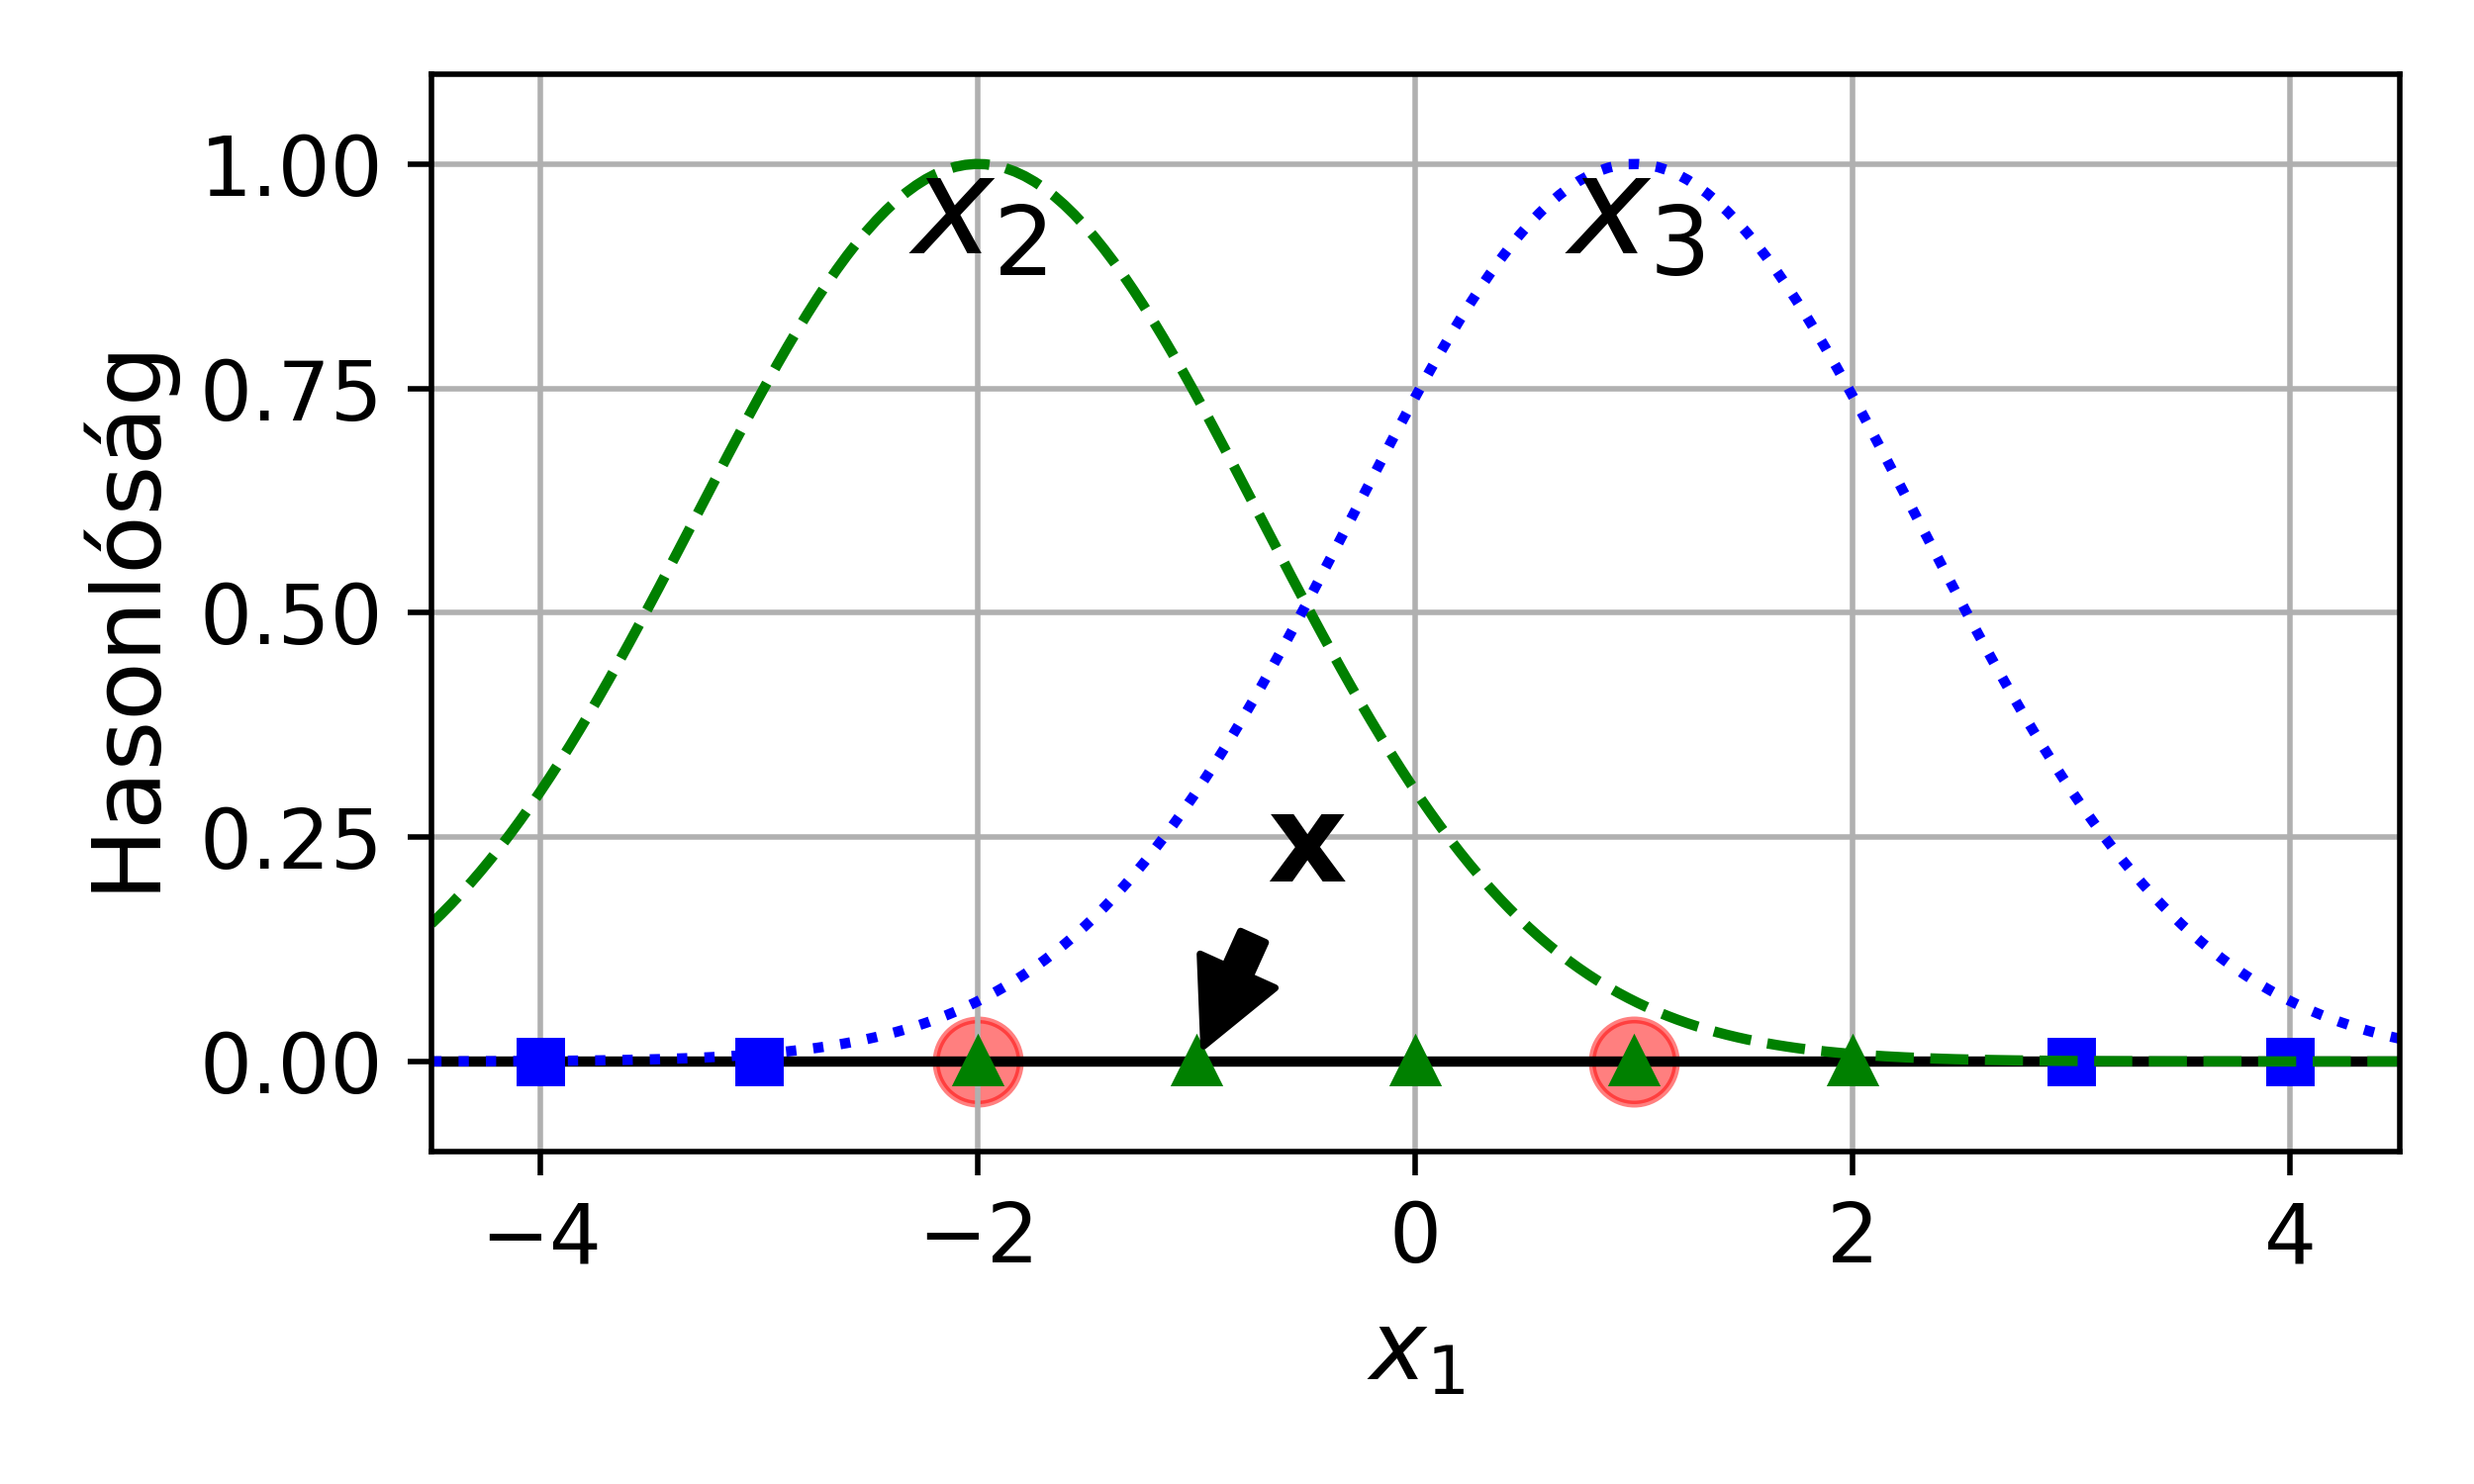
\includegraphics[width=6cm, keepaspectratio]{images/svm_14.png}
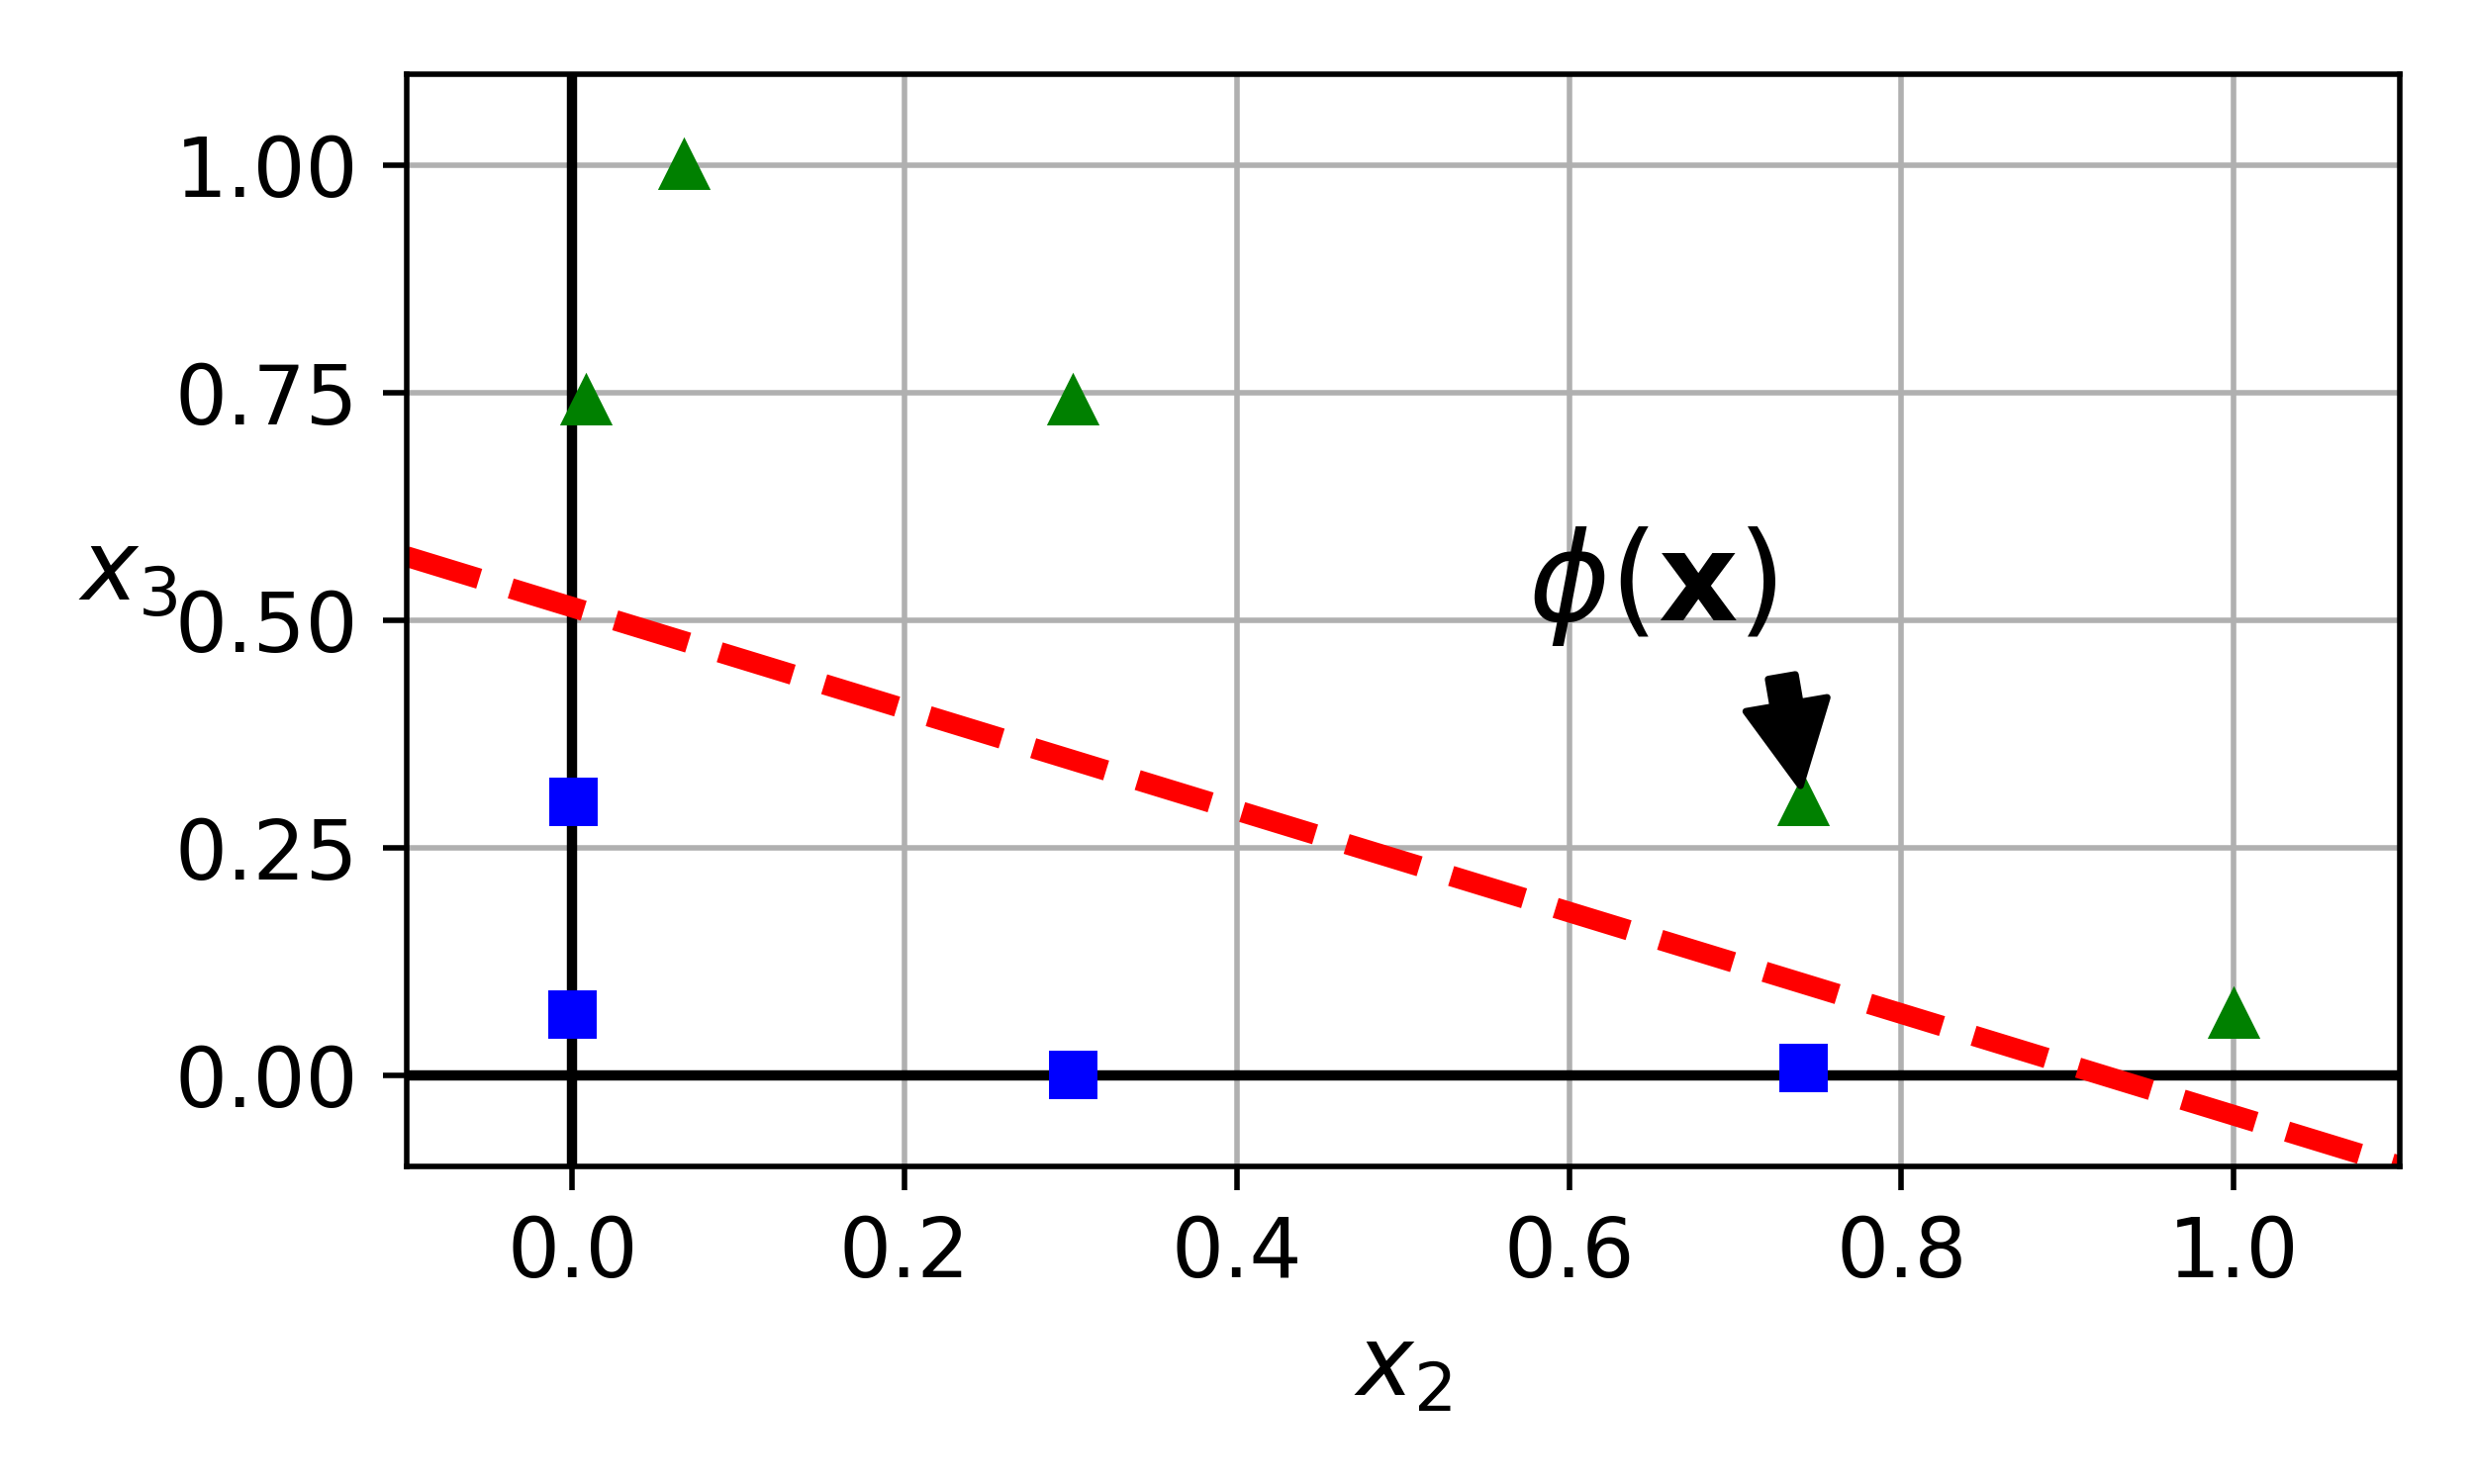
\includegraphics[width=6cm, keepaspectratio]{images/svm_15.png}
\end{center}
\end{column}
\end{columns}
\end{frame}

\begin{frame}{Polinomikus függvények kernelként}
\begin{columns}
\begin{column}{.5\textwidth}
\only<1>{Polinomikus jellemzők hozzáadása alacsony polinomikus szinten nem képes komplex adathalmazokkal dolgozni.\par\medskip
\textbf{Magas szinten viszont nagyon lassúvá teheti a modellt}, mivel minden polinomikus szinten egy külön transzformációt jelent a jellemzőkre.}
\only<2>{\begin{block}{Polinomikus kernel}
A polinomikus kernel transzformáció lineárisan nem szeparálható adathalmazokat transzformál olyan magasabb dimenziós térbe, ahol már lineárisan szeparálhatóvá válnak:
\[
K\left( x,y \right) = \left( \left( x \cdot y \right) + b \right)^d
\]
Ahol:
\begin{itemize}
	\item $b$: A konstans torzítás
	\item $d$: A transzformáció polinomikus foka
\end{itemize}
\end{block}}
\end{column}
\begin{column}{.5\textwidth}
\begin{center}
\includegraphics<1>[width=7cm, keepaspectratio]{images/svm_12.png}
\includegraphics<2>[width=7cm, keepaspectratio]{images/svm_13.png}
\end{center}
\end{column}
\end{columns}
\end{frame}

\begin{frame}{A kernel trükk}
Egy $\varphi$ másodrendű polinomikus leképezés 2D tanító halmazra 3D eredményt ad:
\begin{block}{}
\[
\varphi\left( x \right) = \varphi\left( \begin{pmatrix}
x_1 \\
x_2
\end{pmatrix} \right) = \begin{pmatrix}
x_1^2 \\
\sqrt{2} x_1 x_2 \\
x_2^2
\end{pmatrix}
\]
\end{block}
Ezt a másodrendű leképezést alkalmazva, majd a vektorok belső szorzatait kiszámolva:
\begin{block}{}
\vspace{-.5cm}
\[
\begin{pmatrix}
a_1^2 \\
\sqrt{2} a_1 a_2 \\
a_2^2
\end{pmatrix}^T \begin{pmatrix}
b_1^2 \\
\sqrt{2} b_1 b_2 \\
b_2^2
\end{pmatrix} = a_1^2 b_1^2 + 2 a_1 b_1 a_2 b_2 + a_2^2 b_2^2 = \left( \begin{pmatrix}
a_1 \\
a_2
\end{pmatrix}^T \begin{pmatrix}
b_1 \\
b_2
\end{pmatrix} \right)^2 = \left( a^T b \right)^2
\]
\end{block}
Látható, hogy a vektorok belső szorzata megegyezik az eredeti vektorok belső szorzatának négyzetével:
\begin{block}{}
\vspace{-.1cm}
\[
\varphi \left( a \right)^T \varphi \left( b \right) = \left( a^T b \right)^2
\]
\end{block}
\end{frame}

\begin{frame}{Radiális bázis függvények kernelként}
\begin{columns}
\begin{column}{.5\textwidth}
Ahogy a polinomikus jellemzők esetében, úgy \textbf{a hasonlósági jellemzők esetén is működik a kernel trükk}.\par\smallskip
A diagramon különböző $\gamma$ és $C$ értékekkel tanított modellek láthatóak.\par\smallskip
A $\gamma$ növelése szűkebb haranggörbékkel végzi az illesztést, ezért minden egyed hasonlósági tartománya kisebb. A $\gamma$ csökkentése nagyobb befolyási teret ad a pontoknak. 
\end{column}
\begin{column}{.5\textwidth}
\begin{center}
\includegraphics<1>[width=7cm, keepaspectratio]{images/svm_16.png}
\includegraphics<2>[width=7cm, keepaspectratio]{images/svm_17.png}
\includegraphics<3>[width=7cm, keepaspectratio]{images/svm_18.png}
\includegraphics<4>[width=7cm, keepaspectratio]{images/svm_19.png}
\end{center}
\end{column}
\end{columns}
\end{frame}

\section{SVM regresszió}

\begin{frame}
\tableofcontents[currentsection]
\end{frame}

\begin{frame}{SVM regresszió}
\begin{columns}
\begin{column}{.5\textwidth}
Az SVM regresszió esetében a cél ellentétes az osztályozáséval. A legnagyobb út helyett az algoritmus megpróbálja \textbf{a lehető legtöbb egyedet az útra illeszteni a margósértések minimumon tartása mellett}.\par\smallskip
Az út szélességét a $\varepsilon$ paraméter szabályozza. Nagyon $\varepsilon$ paraméter nagyobb margót jelent. A margón belül hozzáadott egyedek nem befolyásolják a modell definíciót. Ez az $\varepsilon$-érzéketlenség. 
\end{column}
\begin{column}{.5\textwidth}
\begin{center}
\includegraphics<1>[width=7cm, keepaspectratio]{images/svm_20.png}
\includegraphics<2>[width=7cm, keepaspectratio]{images/svm_21.png}
\end{center}
\end{column}
\end{columns}
\end{frame}

\begin{frame}{Nemlineáris SVM regresszió}
\begin{columns}
\begin{column}{.5\textwidth}
Kernelizált SVM regresszorok használata lehetséges regressziós problémák esetén is.\par\smallskip
A következő diagramokon másodfokú polinomikus kernellel tanított SVM regresszorok láthatóak. 
\end{column}
\begin{column}{.5\textwidth}
\begin{center}
\includegraphics<1>[width=7cm, keepaspectratio]{images/svm_22.png}
\includegraphics<2>[width=7cm, keepaspectratio]{images/svm_22.png}
\end{center}
\end{column}
\end{columns}
\end{frame}

\section{Az SVM matematikai alapjai}

\begin{frame}
\tableofcontents[currentsection]
\end{frame}

\begin{frame}{Az SVM működésének részletei}
\begin{columns}
\begin{column}{.5\textwidth}
Az SVM modellek egy $h$ döntési síkot keresnek a térben amelyre:
\begin{block}{}
\vspace{-0.5cm}
\[
h = w^Tx + b = w_1x_1 + w_2x_2 + \ldots + w_nx_n
\]
\end{block}
Attól függően, hogy a mintaegyed a hipersík melyik oldalára esik, lesz beosztályozva a $0,1$ osztályok valamelyikébe:
\begin{block}{}
\[
\hat{y} = \begin{cases}
_{1,}^{0,} & _{ha\;w^{T}x+b\geq0}^{ha\;w^{T}x+b<0}
\end{cases}
\]
\end{block}
A döntési határ azon pontok halmaza, amelyre $h=0$.
\end{column}
\begin{column}{.5\textwidth}
\begin{center}
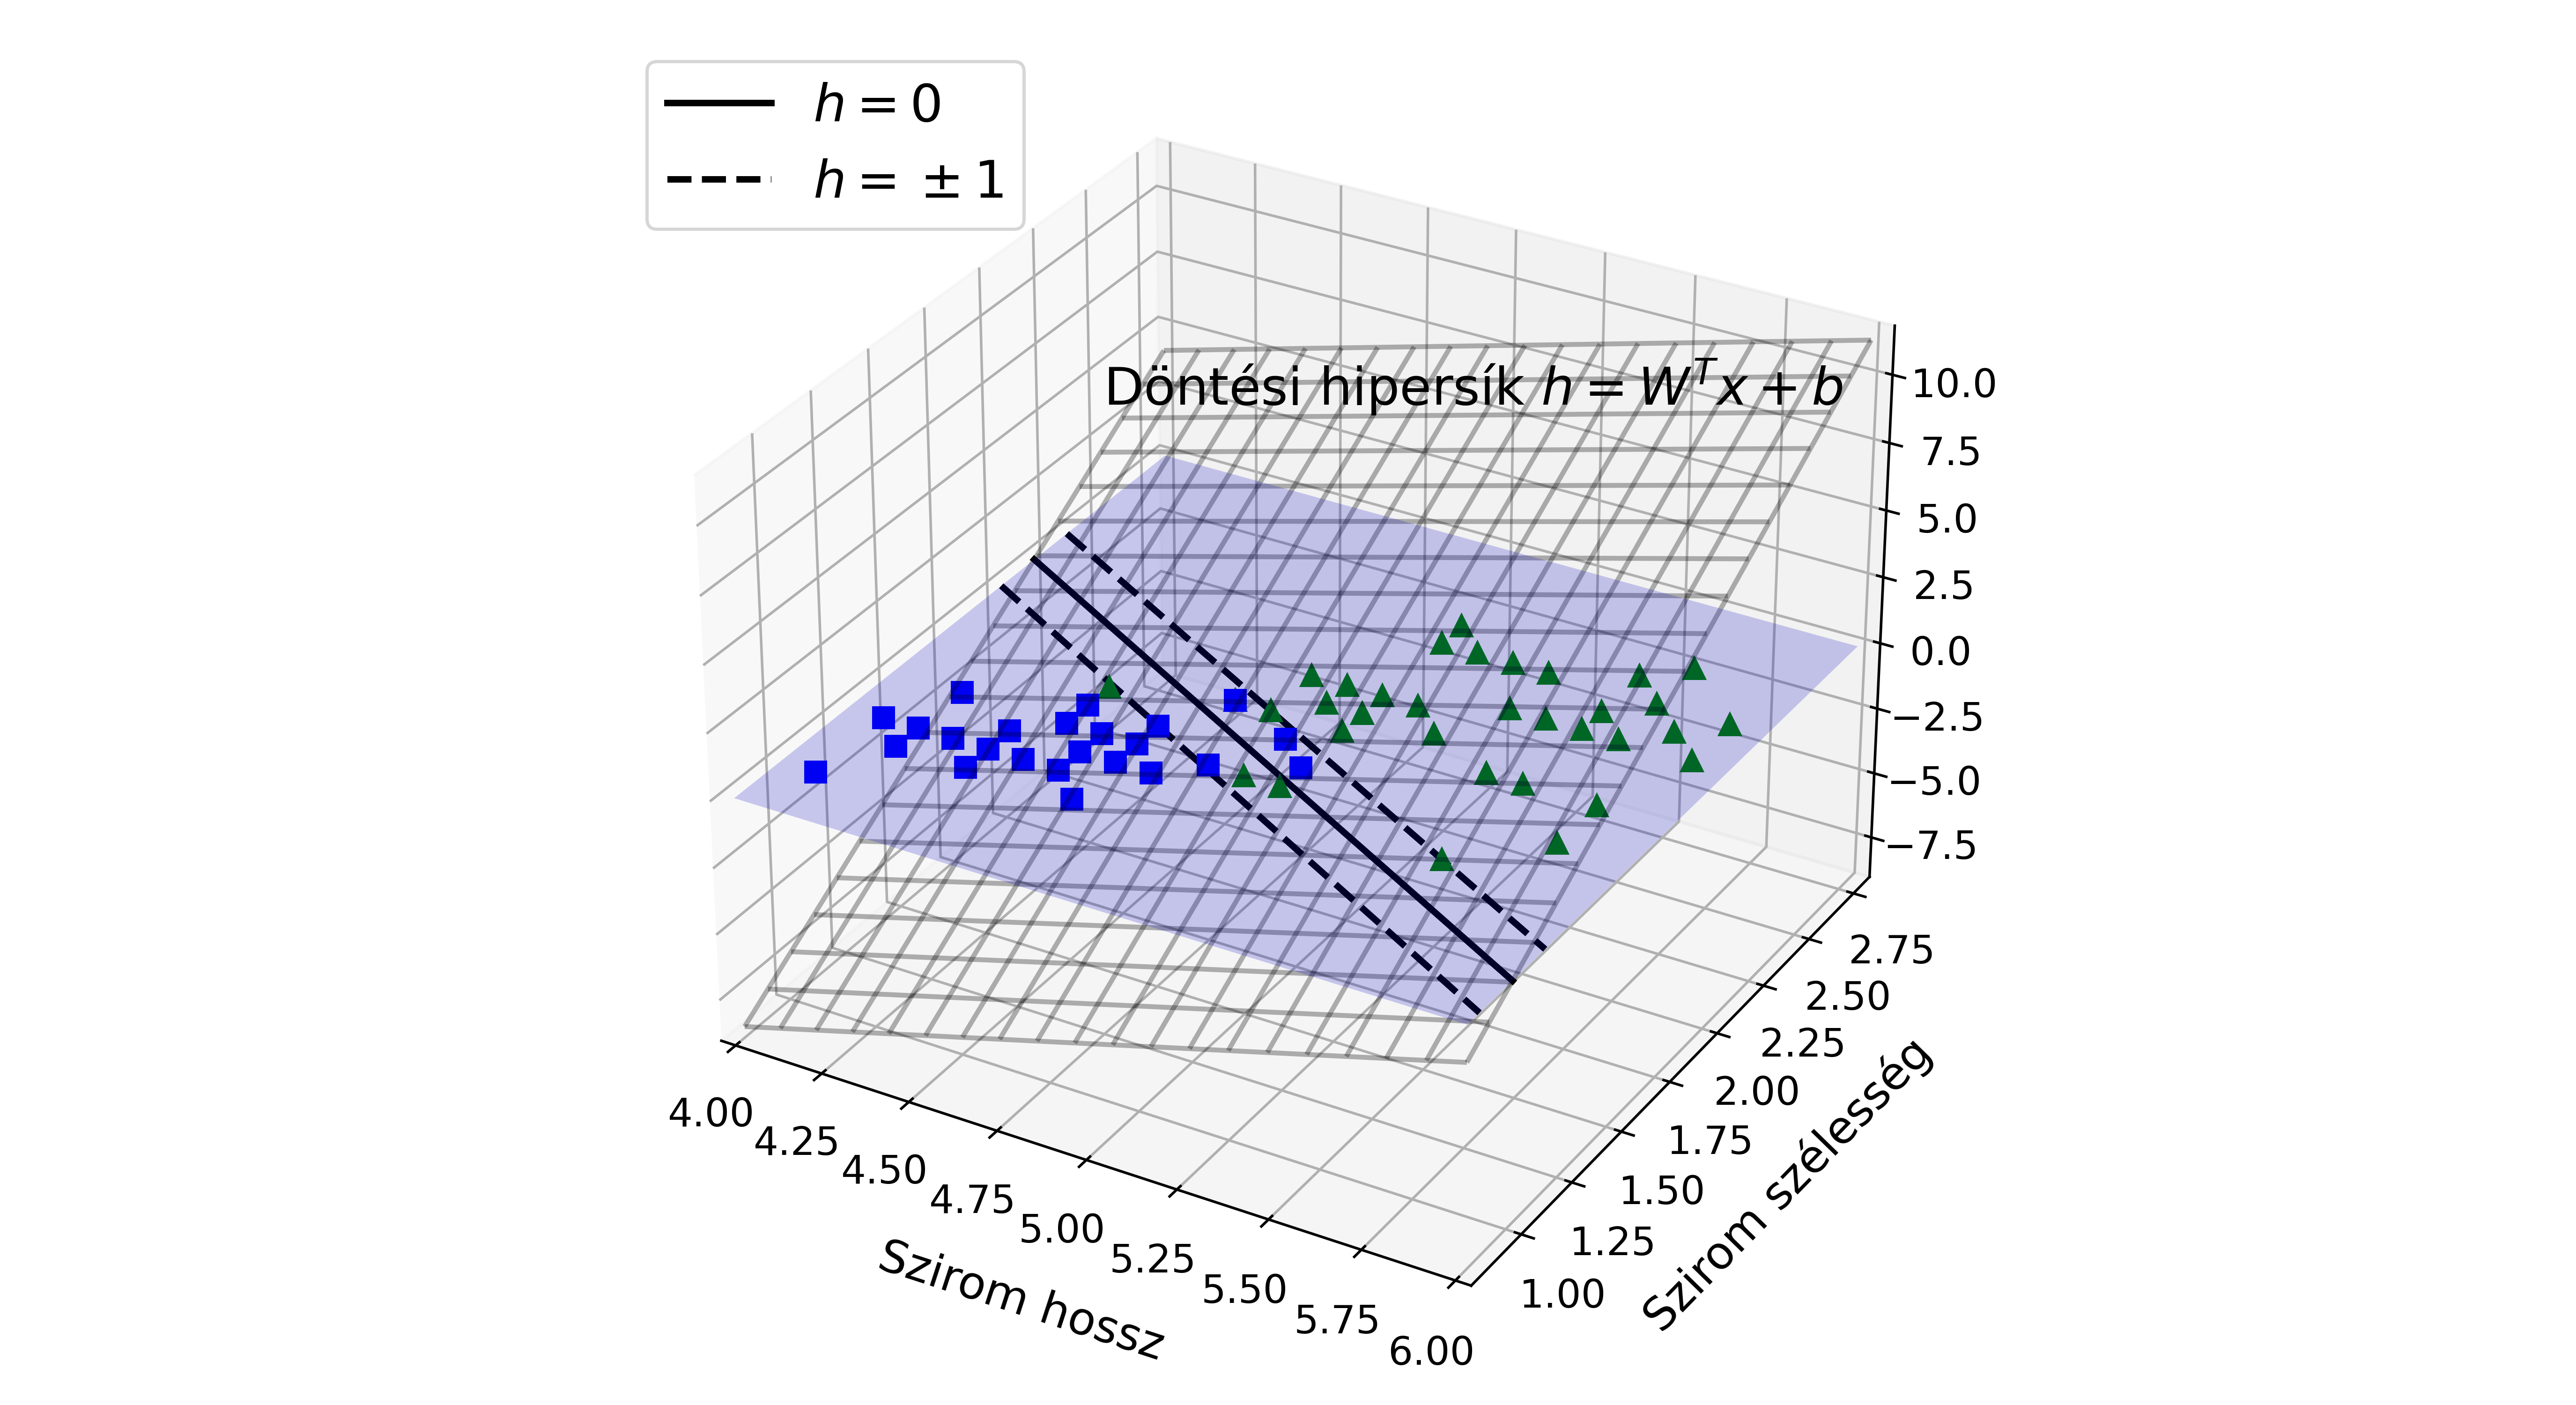
\includegraphics[width=7cm, height=6.5cm, keepaspectratio]{images/svm_25.png}
\end{center}
\end{column}
\end{columns}
\end{frame}

\begin{frame}{A keménymargós SVM célfüggvénye}
\begin{columns}
\begin{column}{.5\textwidth}
A döntési hipersík meredeksége a $w$ vektor normáltja, $\| w \|$. Ez a meredekség fordítottan arányos a margó méretével: nagyobb meredekség szűkebb margót eredményez.\par\smallskip
A célfüggvény a $\| w \|$ minimalizálására irányul annak érdekében, hogy a margó minél nagyobb legyen:
\begin{block}{}
\[
\underset{w,b}{min} \frac{1}{2} \| w \|^2
\]
\end{block}
A következő megkötésekkel:
\begin{block}{}
\vspace{-.2cm}
\[
y_i \left( w_i \cdot x_i + b \right) \geq 1 \; \forall i
\]
\end{block}
\end{column}
\begin{column}{.5\textwidth}
\begin{center}
\includegraphics<1>[width=7cm, keepaspectratio]{images/svm_26.png}
\includegraphics<2>[width=7cm, keepaspectratio]{images/svm_27.png}
\end{center}
\end{column}
\end{columns}
\end{frame}

\begin{frame}{A lágymargós SVM tanításának célfüggvénye}
\begin{columns}
\begin{column}{.5\textwidth}

\end{column}
\begin{column}{.5\textwidth}

\end{column}
\end{columns}
\end{frame}

\end{document}




























